
\documentclass[a4paper,english,titlepage]{article}

\usepackage[T1]{fontenc}
\usepackage[latin1]{inputenc}
\usepackage{babel}
\usepackage{graphics}
\usepackage{graphicx}
\usepackage{haskell}

\newcommand{\todo}[1]{\noindent {\small {\bf todo}}  -- \textsl{#1}}
\newcommand{\hsidnt}[1]{\hspace{5mm}\hsalign{#1}}
\newcommand{\hsalg}[1]{\\ \hspace{5mm}\hsalign{#1}}
\newcommand{\hsdoo}[1]{\hskwd{do}\hspace{2mm} \hsalign{#1}}
\newcommand{\hsdooo}[1]{\hskwd{do}\\ \hspace{5mm}\hsalign{#1}}
\newcommand{\ra}{\rightarrow}
\newcommand{\fn}[2]{\lambda #1 \rightarrow #2}
\newcommand{\uc}{\!\_\!}

\title{DOrcS - Developing Organic (Non-Locomotive) Structures}

\author{Truls Bengtsson \\
Peter Strand}

\begin{document}

\maketitle

\begin{abstract}

Outdoor scenes are increasingly common in computer games today, but
are often very static without evolution or interaction with the
environment. We believe one reason for this is the difficulty of
modelling such scenes with current tools and have developed a system
which conveniently can describe both development and visual
appearance of plants on a high level. 

Two different approaches to plant specifications are explored, both
realized as embedded languages in Haskell, and we provide an application 
which allows both interactive development of these programs and generation
of high-quality visualizations of the resulting plants.


\end{abstract}


\tableofcontents


% Introduction, goals and limitations

\section{Introduction}


    Computer games today drives much of the development in the
    area of computer graphics, both software and especially hardware.
    Producing convincing scenery which mimics the real world as close
    as possible, while still allowing real-time action, is the holy
    grail of the industry.

    Hardware have until recently been the fundamental bottleneck
    behind the visualisation of complex dynamic scenes, thus also
    hindering the development of detailed simulation of events in the
    world. However, the last couple of years the capabilities have
    increased enormously allowing for usage of dynamic and realistic
    visualisations of scenery. Most of these capabilities have been
    used to enhance the main characters of the games, leaving the
    background as dead and boring as before. Much because many games
    take place strictly indoors, or outdoors with limited movement
    possibilities, where a simple background-scene may be sufficient.


\subsection{Plant simulation and visualisation}

    As outdoor scenes becomes increasingly common in gaming scenery,
    so does the importance of representing a visually satisfying
    plant-life. Although some steps have been taken from simple
    texture representations, in order to create a more
    three-dimensional look, plant-life is still often unmixed,
    containing multiple clones of the same model. An outdoor
    environment is seldomly, and then merely scarcely affected by the
    forces and constraints of nature and time, which renders the
    experience only half-living. And the passing of time is, without
    any exception that we are aware of, never taken into account.
    Clearly, it is desirable being able to observe the change of
    seasons and withering of time and limitation of resources.

    Thus we wish to create means to design the plant-life for
    environments supporting such properties. The resulting plants will
    be physically individual and evolve from seed to fully grown trees
    or plants over time. They should respond to changes in available
    resources and strive for their energy source (e.g. the Sun).
    Furthermore, complete environments (e.g.  woods) can be grown in
    realtime during gameplay.


\subsection{Our goal}

    The language we aim to develop should be capable of making
    specifications with enough detail to make convincing models of a
    wide variety of real and imagined plants, both as static
    visualisations and dynamic simulations.  Attributes of the plant,
    both visual appearance and behaviour over time should follow the
    specifications as closely as is desirable. 

    To execute these specifications an interpreter is developed, which
    evolves the plants and visualizes the result. The interpreter is
    also capable of exporting the model to external programs (such as
    ray-tracers), or being used as part of one via a plugin-interface.
    The latter enables 3d-modelers such as Maya or SoftImage to use
    our system to evolve a plant which is then freezed and can be
    finetuned by the modeling-tool.

\subsection{Limitations}

    \label{highlevel_limitations}    
    The focus are set on the graphic result of the simulations.
    That is, we are not attempting to resemble nature in any
    other ways than those affecting the visual appearance of the
    objects. 



% Existing approaches

\section{Background}

    A fundamental aspect of nature is that structures grow by applying built-in
    rules and adapting to circumstances rather than being constructed directly
    in a final state. It is very hard to get around this property, at least if
    we want to produce a large variety of organisms from the same base where
    the final configurations are different and adapted enough to appear
    convincing in their environment.



\subsection{Existing approaches}

    A number of system and approaches exists for modeling and evolving
    plants and other biological structures, most of them are based on
    Lindenmayer systems, described below. 



\subsection{Fractal properties}
    A common question about this project has been that of whether fractals are used.
    In order to answer that, an attempt is made to explain
    very briefly what a fractal actually is.\\
    Mathematically, the concept of a fractal dimension of a
    set is based upon the Housdorff-Besicovitch dimension,
    which is defined using the Hausdorff measure. It involves
    calculating the minimum number of a certain kind of sets
    required to cover the set of interest. There are
    heuristic ways to calculate this, amongst them the
    self-similarity dimension that makes use of the scaling
    property of a measure.\\
    A simpler and more popular way to define fractal is to
    say that it is "a geometric pattern repeated on every
    scale and so cannot be represented using classical
    geometry."\\
    Although somewhat dim, we could say that our trees hold
    some fractal properties, since they would appear when
    looked upon from a reasonable distance, to possess such
    repetetive patterns. These could be further extended by
    setting the the shapes of the branches to an intricate
    self-similar function.
 




\subsection{Lindenmayer System Introduction}

\label{lindenmayer}

    Aristid Lindenmayer proposed L-systems as a mathematical
    formalization of biological development in 1968. They have since
    been successfully used in computer graphics to generate realistic
    models of plants. 

    L-systems build on a very simple idea, successive rewriting of a
    string of symbols where the rules are applied in
    parallel\footnote{A similar system is Chomsky grammars, but the
    rules in these are applied sequentially, which does not reflect
    the parallel workings of nature as well as L-Systems.}.

    An L-system is described by an alphabet of symbols, a starting
    symbol and a number of rules. Originating from the starting symbol
    a string is built by applying matching rules iteratively.

    Consider the alphabet ${ab}$, starting symbol $a$ and rewrite
    rules ${a\rightarrow ab, b\rightarrow a}$. This successively produces the strings: 
    $a$, $ab$, $aba$, $abaab$, $abaababa$, \ldots 

    Now, of what use is strings of letters to model nature?
    The trick is to interpret the string as a geometrical description,
    one common way, but by no means the only one, is to use turtle graphics
    where symbols are interpreted either as lines to be
    drawn or commands to change orientation, simplified.

\begin{figure}[h]
\centering
\caption{Simple L-system }
\label{lsys-example}
\end{figure}
    
    Example \ref{lsys-example} is a D0L system, deterministic, context free
    (taking 0 neighbours in account), L-system. In context dependent
    systems (D$N$L) a rule may take a number of neighbouring symbols
    into account when deciding if it matches or not, however only a
    single symbol is rewritten.


\subsubsection{Parametric L-systems}

\label{param_l_system}

    In parametric L-Systems a number of parameters and
    conditions on these are also included in the rules, allowing for
    simpler descriptions of what would otherwise be quite
    incomprehensible (parameters can be simulated by extending the
    alphabet).

\begin{figure}[h]
\centering
\begin{tabular}{cc}
\multicolumn{2}{c}{
$ \begin{array}{lll}
\omega : & A(100,\omega_0) \\
p_1    : & A(s,w) : s \geq \mathit{min} \rightarrow & !(w)F(s) \\
 & & [+(\alpha_1)/(\varphi_1)A(s \cdot r_1, w \cdot q^e)] \\
 & & [+(\alpha_2)/(\varphi_2)A(s \cdot r_2, w \cdot (1-q)^e)]
\end{array} $ } \\
\\

\includegraphics[height=1in]{images/lsystem1} &

\includegraphics[height=1in]{images/lsystem2} \\
\end{tabular}
\caption{Parametric L-system (using notation from
\cite{lsys_theory_vis}) and possible visualizations, for two sets of
parameters}
\label{param-lsys-example}
\end{figure}

\subsubsection{Further extensions}

    Originating from this very simple idea, the L-systems have been
    extended and improved to support several interesting features such
    as signaling and bug-attacks. However, they tend to get
    complicated to grasp as they grow in complexity. One idea early on
    was simply to write a shell around this framework, to make it
    easier and more intuitive to use. It was however concluded that
    this approach might have caused unnecessary limitations. Instead
    it was agreed to begin at a higher level and perhaps later export
    to L-systems syntax.






% Overview of our solution(s)

\section{Overview}

    This section contains a short overview of our approach to plant
    simulation, focusing on high-level motives behind the design.


\subsection{Realism}


    To catch the immense complexity of real plants i an actually
    usable system would be impossible, since that would require
    simulation at least on the level of individual cells. To reach
    manageable complexity we work instead on the level of major parts
    of a plant, such as a branch or a leaf. While not completely
    realistic from a biologic viewpoint, our simulations are capable
    of producing visually convincing plant models, both static and
    animated.


    The challenge is to find the aspects of nature which are relevant
    for the result of the models, to find a level on which processing
    time is acceptable and yet the appearance implies an underlying
    natural regulating system.
    
    The relevant forces of nature have been separated and
    collected in a set which is deployed on the tree during each
    step.


\subsection{Simplifications}

    In addition to working on a rather high structure level, we make a
    number of other simplifications regarding the nature of biological
    plants. 

    Physical limitations are one aspect which is very expensive to
    account for exactly (since that would require detailed
    calculations of geometric appearance in every step of the
    simulation), but also of surprisingly little importance to
    realism, hence we allow ourselves to break physical restrictions
    either only during parts of simulation, or completely.








% % Nedan �r inte helt implementerat �n, men jag har t�nkt g�ra det.. - peter
% 
% \subsection{Environmental factors}
% 
% 
%     To make the biological complexity manageable the model is kept very
%     simple, while allowing for a few interesting interactions with the
%     environment.
%     The environment of the simulation is approximated by four
%     factors, temperature, sunlight, substance levels and physical
%     structure of the surroundings.
% 
%     Some or all of the environmental factors may vary over time. 
%     Either because of external changes such as different seasons or
%     internal changes caused by the actual simulation (shading, water
%     consumption, collision between large branches, ...)
%      
% 
% \subsubsection*{Temperature}
% 
%     An average temperature for the global world is maintained, local
%     changes are not taken into account.
% 
% 
% \subsubsection*{Sunlight}
% 
%     Each point in the world can be queried for the direction towards
%     the sun and the intensity of the light. Since these properties
%     changes wildly even for shorter periods, they may be approximated
%     either by a simple average or a sampling of real values which 
%     are adapted for the simulation.
% 
% \subsubsection*{Substance levels}
% 
%     (currently only an generalized``power'') \\
%     Each point in the world, air as well as soil, can be queried for the
%     concentration of power available for consumption by the plant.
%     This generic ``power'' can of course be split up in a number of
%     resources such as water and minerals to allow for more detailed
%     simulations, if need arises.
% 
% 
% \subsubsection*{Physical structure}
% 
%     Each point in the world can be queried whether it is free (in
%     the air) or contained by some structure (soil, rocks,
%     plants...). To guide the simulation a vector pointing towards
%     the closest surface to a given point is also available. 
% 
% 
% \subsection{Feedback and limitations}
% 
%     As mentioned above, an extremely detailed model of the world is
%     not realistic in a realtime simulation, especially modifications
%     of the environment caused by the simulated plants is heavily
%     simplified. Water levels and light is accounted for in big blocks,
%     shading is very limited and coarse, small structures are ignored
%     for collision detection, and so on...
% 
%     However, even rather simple models give rise to quite natural and
%     interesting behaviour of the simulated plants.
% 
% 


% General details of our implementation




\section{System design}

    This section describes the overall design of the simulation system
    and the ways in which it can be used, as well as some notes
    regarding its implementation.


\subsection{Overview}

\begin{figure}[htb]
        \centering
        \includegraphics[width=12cm,angle=0]{images/system_overview}
        \label{fig:sys1}
    \caption{Overview of the system}
\end{figure}


    The major part of the application consists of two modules, the
    simulation engine and the visualization module. The simulation
    works on an abstract representation of the plant structure which
    contains necessary information to both control the simulation and
    to enable the visualization module to generate an geometric
    representation of the simulated plant. 

    The abstract geometric output from the visualization module can
    then be used as input to a renderer backend, we have implemented
    two such systems, one for real-time visualizations using OpenGL
    and one for batch generation of high-quality images using Povray.

    The level of the abstract geometric representation is chosen high
    enough to allow for a number of different rendering techniques
    while still making it possible to describe the structure in
    sufficient detail.


\subsubsection{Model}

    In the modeling stage a seed is constructed using one of the
    supported embedded languages.


\subsubsection{Loading}


    The textual representation is transformed into internal
    representation by a compiler and a loader. By using the same language
    in both model descriptions and the implementation of the
    system we get this functionality for free.


\subsubsection{Simulation}

   The simulation engine initializes the internal representation from
   the seed constructed from the model, and iteratively modifies this
   representation according to inputs given by the user representing
   the environment of the simulation.


\subsubsection{Visualization}

    When an visualization is demanded, the internal representation is
    traversed and an abstract geometric representation is constructed. 
    Currently a number of primitives for building
    branches and leaves are available, but this set can easily be
    extended if support for more advanced structures is required, such
    as flowers and various forms of fruits.

\label{system:geomrep}


\subsubsection{Renderer}

    The renderer provides a visual representation of the abstract
    geometry by translating it into either OpenGL commands or a format
    understood by a raytracing system, such as Povray. Many different
    rendering technologies may be used here, the two provided can be
    seen as examples of the possibilities.


\subsection{Implementation}

    The system can be used in two ways, either as a standalone
    application used to develop models in an interactive way, or as an
    embedded library in another applications (a game, for example).
    The standalone applications provides a simple graphical interface
    where the user can develop programs and watch the resulting plants
    interactively. 

    There are two interfaces available for embedding, either the
    abstract geometry is used and parsed by the host, or our
    OpenGL-renderer is used directly. The former approach is
    recommended for serious use since it gives full power to the host
    regarding presentation and rendering decisions.


\subsubsection{Tools}
 
    The simulation modules and development environment is implemented
    using Haskell and ghc together with a number of libraries. A
    number of extension to pure Haskell98 are used, either for
    performance reasons (the ST-monad in one of the approaches) or
    programmatic convenience and abstraction purposes
    (multi.param.type classes, implicit parameters and existential
    types).

    The GUI is written with gtk+hs using HOpenGL for visualization of models. 

    Povray\cite{povray} is used for raytraced renderings.

\subsubsection{Language choice}

    Haskell was chosen for a number of reasons, mainly because we
    know it well and thought it was very suitable for our purpose
    (quick prototyping, ease of abstraction, embedding domain specific
    language, ...)


\subsubsection{DSELS}

    Much have already been said about advantages and disadvantages
    of embedding a domain specific language in an already existing host
    language, we have largely arrived at the same position
    with a few additions, one advantage not mentioned very often, at least
    not explicitly, is the ease of which functionality can be moved back
    and forth between the host implementation and the embedded part.
    This is of great help especially when the problem is a bit fuzzy, when
    we do not know exactly which functionally is needed in the embedded
    language. A pure domain solution which is found to be generally
    useful, or in need of optimization only possible in the core, can be
    directly considered to be part of the language, since the host and
    the embedded parts are the same.







% Detailed description of the monadic simulation engine

% Two-pass algorithm, the passes are independent in the
% sense that the can be respectively turned of during a
% cycle.  But not in parallel, due to enumeration-changes
% caused by sharing, unless these changes are kept in a
% mapping.
% 
% First pass, simulation, runs the programs and updates the
% state, calculates new sharing.
% 
% Second pass, geometrication, evaluates shape functions and
% calculates orientation and position based feedback.
% 
% Feedback means coupling the engine with programs, not
% optimal. 
% 
% 
% 
% The sharing of nodes must be found cheaply, since it's
% potentially run very often. Hence comparisons of explicit
% representations of programs, with potential loop
% detection, is probably to expensive.  Instead labelling
% and a few extra operations are used to find applications
% of already evaluated programs.
% 
% We do not want to evaluate programs fully to compare them!
% 
% Sharing may depend on arguments, not only functions, hence
% it's hard to recalculate it fully. 
% 
% Comparison to Fran \& Pan.
% 
% Discrete with interpolation, gives us something simple and
% faithful to our L-system roots while still allowing smooth
% visualisationa.  Also way more efficient than simulating
% more often.
% 
% Implicit monadic structure => extremely simple, easy to
% move functionality between sim.engine and programs.  Once
% the optimal interface is found => move to explicit
% structure, allows better analysis and also compilation to
% lowlevel language. 
% 
% Feedback loop, necessity? Location independence
% compromised?  Global resources (light -> shadows).
% Glob.res. => sim.engine no longer independent of programs.
% Not much to do unless its implementation can be moved to
% the programs, which makes it hard to make nodes sufficient
% independent, where to store the lightbox?
% 
% 
% 
% Conflicts as a result of sharing and hashing, internal
% state not completely hidden. 
% 
% Global resources, account for readings of these, include
% in hashing if used. Or: let a node mark itself as
% independent of a resource. If explicit embedding is used,
% this can be inferred (at least partially).
% 
% 
% A Node. Defines shape, geometry, program. 
% 
% 
% Disallow update of shape?  .. nah
% 
% 
% Suspend until what? Time. Event? 
% 
% It's tempting to move towards event-driven programs, but
% do we really want that?
% 
% What is a step? Program => execute a number of statements
% or react on input?
% 
% 
% Animation, interpolated discrete vs. continuous.
% 
% 
% Possible underlying models, (event, imperative, dna,
% functional, ...) Short discussion and motivation of the
% chosen way.
% 
% 
% Self-similarity on different levels => not shared here.
% 
% 
% Monadic, Leibniz.
% 
%  Weave programs, with shared or individual state.
%
%







\section{Monadic Approach}



    This approach to simulation of plants is heavily influenced by
    Lindenmayer systems described in section \ref{lindenmayer}, but
    with a number of important differences.  As with L-Systems, a
    plant is composed by a number of smaller parts where each part
    grows by either changing its appearance or creating new parts,
    according to a number of rules or instructions.
    However, where an L-System separates the rules from the passive
    symbols, we view them as a single whole, each symbol is extended
    to a unit containing the rules that governs its development.

    This shift in perception, from symbols and rules to
    instruction-containing parts, was the main idea behind this
    approach, with the hope of making it easier both to describe,
    and to combine, high-level behaviours without losing the
    conceptual simplicity of L-Systems.


\begin{figure}[hbt]
    \centering
    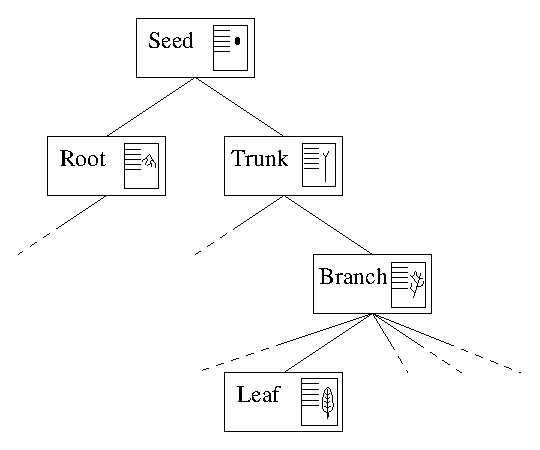
\includegraphics{images/tree_overview}
    \label{monadic:tree_overview}
    \caption{Overview of the internal structure of a simulated tree}
\end{figure}

\subsection{Design Goals}

    A number of design goals lies behind this approach and has guided
    its development, later sections will refer back to these to
    provide motivation for decisions without obvious solutions. These
    are the result both of the initial visions of the system, and much
    experimentation with various simulation cores, given the outlines
    of this approach. Note that they should be seen as guidelines
    rather than rules set in stone, indeed we do break some of them in
    the interest of making something more useful.

\begin{description}
\item[Genericity]
    The core of the simulation engine should be kept generic, without 
    any specific knowledge of things that does not concern its
    functionality, which should be kept minimal. Instead, encode as
    much as possible in the programs in the structure parts.
\item[Independence]
    If parts of a plant only knows very little about each
    other, they are easier to reuse, easier to reason about in
    isolation and it is simpler to discover sharing (see
    section \ref{monadic:sharing}).
\item[Simplicity]
    Only the functionality actually used in a certain part
    should be involved during simulation, no ``dead weight'' or
    default values or programs.
\item[Efficiency] 
    It should be possible to simulate a large number of
    complex plants quickly, preferably in real-time.
    We also want to share representation of similar
    structure parts, this will have lots of consequences for
    the design..

\end{description}

\subsection{Overview}


    A simulated plant is represented as a number of nodes where each
    node corresponds to a major part of the structure of the plant,
    such as a branch or a leaf. The nodes contains all information
    necessary to further their development, visualize them and decide
    when to spawn new subnodes.

    In addition to the actual nodes, which will be dealt with in
    section \ref{monadic:node_internals}, a simulation module and a
    geometry module completes the design. The simulation module
    is responsible for executing the programs in each node, creating
    and destroying nodes upon request and distributing messages. The
    nodes are contained in a tree formed to correspond to their
    relative placement in the plant (see \ref{monadic:tree_overview}). When
    desired, the geometry module traverses the internal structure
    and translates it into a geometrical representation understood by
    the main visualization system (see \ref{system:geomrep}).

    The division in two rather independent passes, simulation and
    geometrification, provides two interesting features:
    When simulating a new world to a given state without
    caring about visualization (until finished), the
    first pass may be run much more often than the
    second, trading accuracy for speed (the visualization
    may be used to calculate feedback originating from
    spatial orientation, which is not directly known in the
    structure tree, more on this in section
    \ref{monadic:feedback}).

    When visualizing a "constant" world (time changing slowly, or not
    at all), the second pass can be used to apply small mutations to
    the model, to give the impression of windy circumstances (rattling
    leaves, bending branches) and also to add detail and
    irregularities.

    The second pass is also used to interpolate between discrete
    states, thus providing smooth animation support cheaply
    (see \ref{monadic:animation}).


\subsubsection{Simulation}

    The simulation code traverses the tree and runs the programs
    associated with the nodes, updating the internal states of all
    nodes and reacting to their behavior. Apart from changing its
    internal state, a node-simulation can have a number of external
    actions: new structure parts may be created, messages can be sent
    to the children or the parent and a node can trigger its own
    death.

    A creation action inserts a new node as a child of the simulated
    part and its program is evaluated once to initialize its state.

    When a part decides to die, itself and all its children are
    removed from the tree.

    Message passing is described in section \ref{monadic:messages}.


\subsubsection{Visualization}

    \label{monadic:viz}

    The shape of a structure part is specified by a function, $ t
    \rightarrow (w \times \mathbf{p}) $, defining the width $w$ and position
    $\mathbf{p}$ along its length $[0..t]$. The parameter $t$ is
    initialized to zero upon creation and the program in each node is
    responsible for updating it according to its development.
    But shape alone is not enough to generally visualize a plant, the
    exact geometry which should be generated must also be specified,
    and this is done by a function parameterized over both the
    parameter $t$ and the shape-function: $ t \rightarrow
    (t \rightarrow (w \times \mathbf{p})) \rightarrow
    [\mathit{geometry}] $. A number of geometric primitives are
    available, such as cylinders, cones and splines (for branches) and
    textured surfaces (for leaves). These are further described in
    section \ref{system:geomrep} and the set of primitives can quite
    easily be extended to allow modelling of more complex parts
    (flowers, for example). 
 
    These three components are stored in each node and may be updated
    during its development, but the shape and geometry functions are
    usually only assigned once upon creation. The presentation above
    is slightly simplified, in addition to the parameter $t$ the
    functions may refer both to the internal state of a node and its
    orientation, the former to allow the shape to depend on more than
    a single parameter and the latter be able to take gravitation into
    account. 

    The complete geometrical representation of a plant is simply
    generated by traversing all nodes and collecting geometry from
    each one of them, using $\mathit{shape}$ functions to get the
    relative placement between the resulting structure parts.


    This model may seem unnecessary complex, why not just have a
    single function returning geometric representation directly:
    ($ \mathit{node} \rightarrow [\mathit{geometry}] $)? 
    The introduced complications can be argued for as follows:
\begin{itemize}
\item We must know where to place subnodes on a node, this could be
        done by storing the exact coodinates but this has the disadvantage
        that they must be fixed for the whole life-time of a part
        unless a possibility to update them is available. Instead,
        each subnode stores the value of the parameter $t$ which was
        current when it was created, and when we need to place a
        subnode we just apply the $\mathit{shape}$-function to it.
        This keeps all shape-related functionality in one place.

\item Subnodes should be placed on the
        surface of the parent, not in the center, thus we need to know the
        width along a nodes extension (think of placing leaves on a branch).

\item Orientation is not known during simulation, but we do want to
        take it into account (bending branches due to gravitation),
        thus we need this as a parameter as well (a vector pointing
        down, in the nodes local coordinate system, is actually
        enough) and this is provided during generation of geometry.
        Note that it is actually impossible to know the orientation
        during simulation if we also want to share nodes (see
        \ref{monadic:sharing}), because a single node may have several
        parents and thus several orientations at once!

\end{itemize}


    A number of convenience functions are available, making
    specification of appearance much simpler than the above
    description may give the impression of.


\subsection{Node Internals}

\label{monadic:node_internals}

    A node manages, in addition to the parameters describes in the
    preceding section, its program and an internal state which can be
    updated and queried by the program. The programs are constructed
    by combining a number of core operations, either sequentially or
    in parallel. Normally a specific behaviour is coded as a sequence
    of operations and several aspects of a plant's behaviour are
    combined together in parallel.

    The operations are described by small example programs, to give a
    feel for how they are used rather than just specifying syntax.
    Note that the language is not very stable at the moment, details
    may change.


\subsubsection{Core Operations}

    The power of this approach lies in the possibility to build
    libraries of higher level operations out of the quite small number
    of primitive operations described in this section. 

\paragraph{Appearance}

    The components described in section \ref{monadic:viz} can be
    assigned by the following instructions:

\begin{haskell*}
branch = \hsdooo{
        shape (\fn{t}{(0.1, {\bf e}_y `scaled\!\_\!by` t)}) \\
        geometry (mk\!\_\!branch brown) \\
        set\!\_\!pos 1}
\end{haskell*}
The above program specifies a brown branch, following the
y-coordinate axis, with a constant length of one.

Not very interesting though, it doesn't grow. To do that we need to
update the position each step.

\begin{haskell*}
init\!\_\!branch = \hsdooo{
    shape (\fn{t}{(0.1, {\bf e}_y `scaled\!\_\!by` t)}) \\
    geometry (mk\!\_\!branch brown)} \\
grow\!\_\!by g = \hsdooo{ 
        p \hsfrom get\!\_\!pos \\
        set\_pos (p\!+\!g) }\\
branch = \hsdooo{
    init\!\_\!branch \\
    loop (grow\!\_\!by \ 0.1) } \\
\end{haskell*}

The \emph{loop} function runs its argument over and over again,
until \emph{stop} is encountered.
\begin{haskell*}
branch = \hsdooo{
        init\!\_\!branch \\
        loop \$ \hsdoo{
            grow\!\_\!by \ 0.2 \\
            p \hsfrom get\_pos \\
            when (p\!>\!1) stop
        }}
\end{haskell*}

    We have already seen a number of interesting properties of the
    language, thanks to being embedded in haskell we get a lot for
    free, especially the ability to abstract out common functionality
    in reusable functions.


\paragraph{Spawning}

    To create substructures the functions \emph{spawn} and
    \emph{spawn\_ori} are used, the former keeps the orientation
    of the parent while the latter allows arbitrary rotations to be
    applied.

\begin{haskell*}
leaf = \hsdooo{
    shape (\fn{t}{(t,{\bf e}_y})) \\
    geometry (mk\uc{}leaf (texture ``green\_leaf'')) \\
    loop (get\uc{}pos >\!\!>\!\!= set\uc{}pos . min 1 . (+0.2)) \\
} \\
branch = \hsdooo{
    init\!\_\!branch \\
    loop \$ \hsdoo{
        grow\!\_\!by \ 0.5 \\
        spawn\!\_\!ori \ ({\bf e}_z `rotate` (pi/3)) \ leaf \\
        grow\!\_\!by \ 0.5 \\
        spawn\!\_\!ori \ ({\bf e}_z `rotate` (-pi/3)) \ leaf \\
  }                    
}
\end{haskell*}

This program grows a branch which spawns a green leaf every 0.5 units
of its length, on alternating sides.

\paragraph{Message propagation}

\label{monadic:messages}

    Nodes may interchange messages (currently only strings)
    to propagate resources or signals either upwards or downwards in
    the node hierarchy. One example of usage is to signal leaves to
    fall off synchronized when the parent-branch has run out of
    energy. Messages should only be used when no other options are
    available, they don't fit very well in the model and was only
    added because some problems cannot be solved without them, in an
    acceptably simple way.


\paragraph{Parallelism}

    As mentioned in the introduction to this section programs may be
    combined in parallel as well as sequentially. This turned out to
    be a very powerful abstraction mechanism since it allows different
    behaviours to be encoded as individual and independent program
    fragments.

\begin{haskell*}
stop\uc{}at \ p_{max} = \hsdooo{
    p \hsfrom get\uc{}pos \\
    when (p >= p_{max}) stop
} \\
branch = \hsalg{
    init\uc{}branch \ `weave` \\
    \quad loop (grow\uc{}by \ 0.2 \ `weave` \ stop\uc{}at \ 1.0)\\
 }
\end{haskell*}

    The function \emph{weave} combines two program fragments by
    returning running each of them one step further every time itself
    is run, thus weaving them together.

    But how long is a step? Since the simulation is discrete we must
    have a way to determine how many instructions to run in each
    program each time its node is simulated. This is done by the
    instruction \emph{suspend}, which saves the current state and 
    triggers the execution of the next program in turn.
    Thus \emph{loop} could be implemented as:

\begin{haskell*}
loop m = \hsdooo{
    m \\
    suspend \\
    loop m \\
}
\end{haskell*}

    It is not done this way, due to reasons related to sharing of
    nodes, but it can be thought of the above program in all essential
    ways.
    An alternative to an explicit \emph{suspend} function would be to
    suspend after every instruction, but that would result in
    unnecessary inefficient execution with only a slight syntactic
    gain. And it could be problematic to get a feel for how fast
    different program executes relative to each other.

\paragraph{Local State}

    An arbitrary number of parameters can be stored in the internal
    state for each node, these can be used to implement new operations
    for behaviours not possible with the provided single length
    parameter, for example keeping track of resource levels, mass or
    growth parameters.


\subsubsection{Gravitation}

    To calculate gravitational effects we need to know some
    things we have not considered yet, the density and
    elasticity of a branch and its orientation. The density
    and elasticity can be stored in the internal state and
    the orientation is made available to us by the visualization
    module. Essentially, the shape function is adapted to take these
    effects into account using an sufficently advanced model regarding
    the desired effects. It is worth noting that one can get very far
    with very simple models, appendix \ref{monadic_examples} contains
    a few examples of this.


\subsubsection{Forests}

    The language can not only be used to describe single plants, but
    also groupings of them. Instead of starting with a branch with
    spawns other brances and leaves we start with a meta-node, which
    in turns spawns whole plants places as usual with its
    shape-function (which now defines the surface of the
    forest-covered area).
    To avoid symmetrical and repetetive patterns random numbers should
    be used when placing plants and determining their types.


\subsubsection{L-system simulation}


\label{lsystem_to_dsel}

    Traditional L-system can be simulated by creating one node-type
    for each symbol, containing the parameters for parametric
    L-systems. The rewrite-rules are rewritten as programs which
    updates the state accordingly and spawns new subnodes when
    the corresponding rule would trigger such action.
    
    The plants in figure \ref{param-lsys-example} are generated using 
    the following program, taken from an example in
    \cite{lsys_theory_vis}:

\newpage
\begin{haskell*}
lsystem = \hsdooo{
       geometry (mk\uc{}branch (Flat (0.2, 0.6, 0.15))) \\
       st \hsfrom getst \\
       shape (\fn{t}{(max (w st) 0.01, (down `scaled\uc{}by` 0.6t) + (0,2t,0))}) \\
       loop \$ \hsdooo{ 
         LSys \alpha_1 \alpha_2 \varphi_1 \varphi_2 w_0 min_s r_1 r_2 q s w cs \hsfrom getst \\
         \hscase{(cs < s, s <= min_s)}{\\
          \!\!(\_, True) \ra stop \\
          (True, \_) \ra \hsdoo{
               modst (\fn{s}{s \{ cs = cs + 0.02 \}}) \\
               set\uc{}pos cs 
          } \\
          \_ \ra \hsdooo{
             set\uc{}pos s \\
	     \hskwd{let} new\uc{}child \alpha \varphi r q = spawn\uc{}ori \\\hspace{8mm}\hsidnt{
                            ({\bf e}_z `rotate` \alpha `mulq` {\bf e}_y `rotate` \varphi) \\
                            (\hsdoo{ modst (\fn{p}{initial\uc{}state
                            \{ s=r\!\cdot\!s, w=q\!\cdot\!w \})} \\
                                next plant\uc{}lsystem) }}\\
             new\uc{}child \alpha_1 \varphi_1 r_1 q \\
             new\uc{}child \alpha_2 \varphi_2 r_2 (1\!-\!q) \\
             stop }
         }
       }
 }
\end{haskell*}
    The sequence \emph{next f} is a shorthand for \emph{suspend} followed by
    \emph{f}, \emph{mulq} combines two rotation operations.

    Here we also see the usage of \emph{getst} and \emph{modst} to
    operate on the local state, which type is defined as a usual
    haskell data-type not shown here. An alternative, and simpler,
    interface to the local state is also available, which avoids the
    need to define a new data-type.

    Context sensitive L-system are a bit harder to
    simulate, since the only inter-node mechanism available is
    message-passing each rewrite has to be rewritten as a
    number of steps which first query the surroundings and
    then change node accordingly, no work has been made in
    this area.



\subsection{Feedback}

\label{monadic:feedback}

    During simulation the internal nodes are completely agnostic of
    location and orientation, however sometimes we do want to add
    dependencies on global properties such as sunlight, shadows and
    global resource levels.
    This bookkeeping could be done in an extra pass between
    geometry-generation (the only time when we know absolute positions
    and orientations) and the next simulation pass, by calculating
    appropriate feedback and apply to nodes requesting it.
    (this is work-in-progress.)

\subsection{Animation}

\label{monadic:animation}

    Since this approach uses a simulation algorithm with discrete
    steps, smooth animation it not possible out-of-the-box. However,
    the representation of geometric information has been carefully
    chosen to allow interpolation between states, which allows us
    arbitrary precision of animations without involving the simulation
    algorithm at all. Best results are achieved if the
    programs are written with animation in mind, since the (linear)
    interpolation only works well for small changes in appearance. 


\subsection{Sharing}

\label{monadic:sharing}


    For a tree with, for example, a couple of thousands leaves, it is
    very wasteful to represent and simulate each one of them
    individually, it is quite probable that a large number of them
    will be in a equal or similar state of development at any given
    point in time. To take advantage of this, the simulation algorithm
    tries to find equal or mostly equal structures and merge them,
    thus only simulating and representing them once. This greatly
    improves the performance of big scenes but also put a lot of
    limitations on the implementation, to find sharable parts we have
    to compare the nodes for equality, which is a bit challenging
    since they both contain computations and state of arbitrary types
    (functions, for example, are not comparable in haskell). 

    Two techniques are used to work around this limitation, one is to
    encode functions using an explicit notation as abstract
    expression trees, and another is to use an impure ``hack'' similar
    to the one Koen Claessen uses to discover sharing in circuit
    descriptions in \cite{obs_sharing}.  The former is used for
    shape-functions and the latter for node-programs. This solution is
    not completely satisfactory since it fails to discover some
    opportunities for sharing, but it is just an optimization so the
    only consequence is a slightly slower simulation. This is one
    price we have to pay for using an embedded language in Haskell, we
    do not have access to the concrete programs, only the expressions
    they generates, thus obvious shared references in the
    text-representation of programs are not visibile to us, but
    have to be rediscovered.

    An alternative would be to use an explicit notation also for
    programs, but since they can be quite long, and have to be
    compared often (potentially each simulation step), it was
    considered as a bad tradeoff even if more opportunities to sharing
    would arise. 




% Detailed description of the database-bases simulation engine
\section{Parameterized approach}

\subsection{Introduction}

The Parameterized approach concludes that all plants function the same way on a
certain level and all that is really needed to describe a plant is to set some
parameters for this universal algorithm. A plant would then consist of a set
of parameters. All that is left is to sort out these parameters, find an 
appropriate level and write the algorithm.

\subsubsection{Common tree features}
In order to structure the describing language, common features are sought out.

\paragraph{Levelized architecture}
Plants and especially trees have a strong tendency to possess a level-like
structure. Considering the trunk or perhaps root as the bottomlevel, levels
of branches are applied in a hierarchical order, ending with a toplevel
consisting of leaves. Although it does vary, the number of branchlevels
leading up to a leaf is strikingly constant throughout a grown-up tree. This
probably due to the fact that a leaf with a lesser number of sublevels are
inclined to be shaded from the sun by leaves sprouting from a deeper
branch-hierarchy, since those are likely to be farther out and of greater 
numbers. 

\paragraph{Branchlevel similarity}
Branches belonging to the same level often seem to share a number of
properties, such as growth-angle from motherbranch and spawning statistics. 

\subsubsection{Distinguishing tree features}
As the common features are considered when designing the static parts and syntax of the 
language, the individualizing properties will be reflected upon the dynamic
parameterized parts.

\paragraph{Branchleveling}
Given a certain branchlevel, how often is it inclined to spawn a childbranch
of which sort.

\paragraph{Branchdistributioning}
How much energy does a branch use up on itself and how much does it pass on to
its children.

\paragraph{Branchshape}
Physical shape of the branch.

\paragraph{Treeshape}
The overall impression of the tree's physical shape. Typically columnar, cone,
distributed or blobbed.

\paragraph{Constraints}
Is a childbranch allowed to grow further than the motherbranch, or perhaps no
more than 30\% of the total motherbranch development?

\subsubsection{Meta-language characteristics}
Considering the aforementioned properties of trees, the components of the 
top-level language where decided to be stack-leveled, that is
branch-descriptions are stacked in the order they appear on the tree. A branch 
will spawn all branches which are lower on the stack (the trunk being the top 
element). Stack elements contain an interface which says how that level is
attached to its motherlevel, and a plant node expressing the properties of
instances of the level.

\paragraph{Interface}
The \emph{interface} contains information about \emph{branch distribution}, 
determining the overall shape of that level. \emph{Spawn count}, for instance 
pines may spawn several sprouts at the same time, creating branchrings. \emph{Angle 
distribution}, angle in relation to its mother and the upvector. \emph{Evolution}, 
determines when the level spawns. \emph{Energy modification}, constraints on 
how the level may grow.

\paragraph{Plant Node}
A \emph{plant node} characterizes the \emph{shape} of the level.
\emph{Elasticity}, determining gravitational displacement. Possibly also
\emph{texture} and \emph{size} if the node is a leaf.

\paragraph{}
The seed of a simple tree could be then be thought as a stack of
(interface, node)-tuples:
\\\\
{\bf (trunk interface, trunk node)\\
(branch interface, branch node)\\
(leaf interface, leaf node)}

\subsubsection{Chaotic behaviour of nature}
Regarding nature as a system, it has chaos properties. That is, although in
some sense deterministic, it may require a very large number of variables
with arbitrarily high precision in the equation necessary to calculate 
its behaviour and state. Its
affect on a plant appears to have random properties, yet dominated by major
factors such as temperature and sunlight exposure. This randomness on a
low-level, however suggests that randomness should be employed to work on the
shaping of a tree.

\subsection{Meta language}
\subsubsection{Ambition and structure}
The aim was set to create a language, which on the toplevel would be very
intuitive and easy to use. The branching structure and types would be set with
a set of base-components, which should suffice to create a number of basic
treetypes. Using a set of modifiers and a library of more lowlevel components
the seed can be further modified to a desired behaviour. On the base of each 
seed is an \emph{earth}-component that contains
the root function and other general information. The '<<'-operator simply
binds the branchlevels in a hierarchical order. Conceptual examples
below. 
\\\\
\begin{tabular}{ll}
  &StdEarth\\
  <<&(trunk-interface, pine-trunk)\\
  <<&(ring-interface, straight-branch)\\
  <<&(horizontal-interface, straight-branch)\\ 
\end{tabular}
\\\\
\emph{Basic model of a pine tree}\\

\begin{tabular}{ll}
  &StdEarth\\
  <<&(trunk-interface, modThickness 5.0 \$ pine-trunk)\\
  <<&(modDistribution triangleFunc \$ ring-interface, straight-branch)\\
  <<&(horizontal-interface, straight-branch)\\ 
\end{tabular}
\\\\
\emph{Modifying the basic model of a pine tree. Setting thickness property to
5.0 and the general shape of the tree to a triangular one}

\subsubsection{Language Levels}
\begin{enumerate}
\item
Toplevel language "MetaPlant", a set of combiners and basic factors.
\item
Modifiers with parameter library. Extends the toplevel language.
\item
Lowlevel library components. Buildingblocks for the parameter library.
\item
Host language datatype constructors. Haskell constructs derived from the
toplevel language.
\end{enumerate}

\subsubsection{Randomness}
As suggested above each BranchState contains a random seed, accessible by the
shaper functions which can ensure that branches are given unique
representations.

\subsubsection{Libraries}
There are a set of standard interfaces and standard branches, for typical tree
paradigms, such as leaf and pine trees. These sometimes take a few arguments 
that set the starting growth angle interval, the size and texture of a leaf or
the wigglyness of a branch. These standard components are then modified by
adding replacing properties with modifiers. Typically, one would like to change
the shape of the tree with a new distribution function. The modifier may take
completely new function, but in most cases a constructor-function is used, which only
take some essential parameters and hides away the ugliness of the process. In
the distributor case the essential parameters would be constituted of a function
that takes the development of the branch at a certain place and says what mass concentration should
be at that level. Sometimes the normalized position (position in relation to
entire length) is more suitable, for instance when a tree is supposed to look
the same its entire life (a spruce maybe), where as a function such as (\\rel\_pos
-> 1.0 - rel\_pos) would be deployed (0.0 being near root and 1.0 near the top).

\subsubsection{Limitations}
Although the seed may be extensively configured the heart of the behaviour is
still in the simulation-module which may not be modified. Some things regarding
the life of the plant may thus not be changed. For example, when power is low
the plant will inevitably attempt to sustain the leaves closest to the root and
not the other way around. A branch may not switch plant id (identifying the
internal type of branch). If a branch falls off the tree, it will never grow out
again.

\subsection{Simulation}
The simulation algorithm takes the current state of the tree, an environment
and the time to run. The root-function converts the environment to power that
is sent throughout the plant according to the interfaces of the branches.
\subsubsection{Overview}
Beginning at the trunk the following steps are taken:
\paragraph{Vitalize leaves} 
It is feasible to assume that the trees first priority is to feed its leaf,
since they are essential for the photosynthesis that generates the carbon
substances needful for further development of the plant.
\paragraph{Feed the child branches} 
Power is disposed according to the distribution
function, that determines the overall shape of the plant. Each child is then
simulated recursively with its granted power.
\paragraph{Simulate forces of nature} 
The forces and corrosive powers of nature are taking affect on the current
level.
\paragraph{Evolve this branch}
Use granted power to develop branch and add new
children.

\subsubsection{Preparations}
The environment, including resources, temperature and other peripheral factors
are passed to the simulation step along with the time to run. Each plant then
have a root function, which converts the given environment to the fictive unit
growth-power. Since the power remains static during the simulation step; it is
important that a higher function creates environment-wise fine-tuned intervals
for a believable evolution. Together with the root-function-evaluated power,
there may be unused, accumulated power from previous steps which are added to
the power-pool. To generalize the concept of resources to a single powerunit
might seem limiting, but has proven quite satisfactory and simplifies the
underlying methods. There are even some possibilities to at the bottomlevel
take heed to the surrounding environment, when using a development modification
function, that at the lowest level can modify the development of a branch.\\\\
In the case that it is the first-time simulation-step for the given plant, a
special genesis-path is taken, which setup the infant trunk-level branch with
seed according parameters, the most important being the event list.
\\\\
Further more, before the actual powerdistribution takes place, some flags are
set and the simulation state initialized.

\subsubsection{Power distribution - discussion}
Each seed has at each level a function that says how much of the total
mass on a level should be concentrated to each branch. That is, for each of
the attached branch, a mcn (mass-concentration-number) is generated from the
seeds distribution function on that level. For a pine tree it
would typically somewhat triangular, $f = 1 - x$, where x is the relative
position on the motherbranch $\frac{position}{mothers development}$ and for a tree 
with columnar shape near
constant $f = 1.0$. A strangely shaped tree may wish to use absolute coordinates
to shape sharp and steady contours.
\\\\
Ideally, the power, $p_{incoming}$, will attempt to fulfill:
$p_{incoming}=\frac{d}{dt}(w_{reference} - w_{current})$, with $w_{reference}$
being the mass according to the distribution function and the $w_{current}$
the actual current mass distribution, mass by definition equaled to energy. 
It is however, and for several reasons, impossible to use this formula, the 
functions not being derivable for one thing. Hence, approximations must be
explored.
\\\\
Alot of approaches was attempted in order to find a strategy with the sought-
for-properties. The necessary features includes maintaining the shape defined
by the seed, promoting self-survival and perhaps most difficult - not loosing
any power throughout the distribution flow. 
\\\\
The naive way to distribute would be to simply calculate the
mcn for each subbranch at the current level,
normalize them and multiply with the available power, assuming that all power
will be transformed into mass, in one way or another. There may however be
branches that cannot consume the power given to them, due to restrictions of
strength (or other), then something must be done with the excessive power. 
One strategy is to store the excessive power returned by the children at the 
motherbranch and then simply add it to the incoming power next round. If the 
tree is growing and the distribution depends mostly on relative position (which 
then changes rapidly), this scheme is quite useful, but proves to end up 
accumulating vast 
amounts of power at certain branches is most cases. Countermeasures against
this sort of powertraps may begin with regarding how much power a certain
branch fed the last cycle and adapting the current flow to match if it was
minor. This power limit must however be updated at some point,
since it may very well be that the branch will be able to accept more power
in future times. Thus the powertrap persists. One solution would be to raise
the powerlimit gradually and thereby decreasing the unwanted power buildup.
This, although working with reasonable result introduces uninvited latency to
the system, breaking the distribution model.
\\\\
Another issue one must take into account when contemplating the distribution
is the fact that the prerequisites that determined the current distribution 
change after the new power has been deployed. That is - the calculated
distribution is really only valid for the first infinitesimal bit of power. As
soon it is consumed it changes the mass-distribution and thereby the desired
power-distribution.
\\\\
The perhaps most obvious solution would be simply to chop the simulation
timeframe into very small portions, which well approximates the infinitesimal
criteria. This however is very time consuming, since running the simulation is
a time-expensive operation no matter the distribution issue solved. In stead,
the timeframe partitioning is left to a higher level.
\\\\
The difficulties in not loosing any power has made itself heard on
implementation level.

\subsubsection{Power distribution - working strategy}
Testing of several models with regards to above arguments lead up to a method
working in multiple stages. It is assumed that the timeframe of each
simulation step is relatively short.
\paragraph{Feed to equilibrium}
In the first step, an attempt is made to bring justice to the branches. The
power difference $w_{reference} - w_{current}$ is computed (values clamped to
$[0..\infty]$, we don not want backwards growth). Probing each of the
potential branches (those given a non zero, positive distribution) only those
branches ready to accept more power are selected and then the power
converted to mass is used to neutralize the power difference in those
branches. The probing mechanism is provided by sending some small amount of
power to the simulation functions of the branches, detecting whether it
is bounced back or not. The power sent to the branches may partly bounce back,
should the branched be saturated. That power will be stored and used in the
next step.
\paragraph{Feed the hungry}
Given that any power remains when the assumed equilibrium is reached, the
branches are once again probed, and the remaining power is sent throughout the
hungry branches in accordance with the distribution.
\paragraph{Feed thy self}
The remaining power (including the one rejected in the second step) is used to
evolve the current branch. The power rejected on the current level is passed
back to the superlevel, and if the current level happen to be the baselevel
the power is accumulated and added to the incoming power next time around.
Therefor it is important not to use to great steps or December may become
sunny as June.

\subsubsection{Regulators}
Intuitively it might seem tempting to view the tree as a dynamic system and
deploy regulators to control it. Simplified, the system would then preferably be
represented as the following illustration.

\begin{figure}[htb]
        \centering
        \includegraphics[height=2cm,width=6cm, angle=0]{images/regulsimple}
        \label{fig:db:graph1}
\end{figure}

Here, a PI-regulator would seem fitting to steer the power going into the
current branch.

However, because of the modifier preceeding the branch, the behaviour of the branch 
is not as depending on the insignal as would have to for this to work.

The implemented solution would by similar methods be illustrated as follows.
 
\begin{figure}[htb]
        \centering
        \includegraphics[height=5cm,width=12cm, angle=0]{images/regulsys}
        \label{fig:db:graph2}
\end{figure}

Note how the probe signal ('test' in the figure) opens the feedback loop if the
probe is successful. This is indeed more or less a plain P-regulator, making use
of several ingoing signals to the system.
 
\subsubsection{Evolving the current branch}
Each branch has an event list which includes events with attached development
stamps, stating at which level of development the events will activate. The
events are different sub-branchings, where the branch will spawn off new
branchlings. Thus, in order to evolve a certain branch, the following steps
are taken.
\\\\
\emph{Find development of next event}, by parsing the event list. If that
development is not reached within the given timeframe, then simply grow, else
\emph{grow to the development of next event}, subtract the time used from the
timeframe and start over seeking the next event. When the algorithm is
restarted, only the newborn branches are taken into account. The leaves of the
branch is naturally only fed during the first round. 
\\\\
Growing is done by
converting the integrating the power over time and then adding the resulting
mass/development/energy to the current development. Before it is added, the
branch has a chance to use its \emph{development modification function} to
limit or boost the development being added. The typical use being
not to allow a branch to grow longer than its mother has since the
branched was spawned off. It could also be used to encourage certain shapes.

                       
\subsubsection{Creating a new branch}
To spawn a new branch \emph{b} from an event at branch \emph{a}, the seed is inquired of possible
sublevels and at which time they will branch from \emph{b}. These events are
stored in \emph{b}'s eventlist. Other properties such as growth angle, growth
shape are computed and stored. At \emph{a}, the next \emph{b} event is stored.
\subsubsection{Leaves}
Leaves are treated separate from branches, since they do not require the same
care as do the branches. When a leaf has been born, it prospers until the
power is reduced beyond a certain level beyond which it starts to fade away.
When the leaf has faded completely it will fall off the tree. A branch with no
leaves on it will also subsequently fall off the tree. As spring of power
comes, a new leaf will appear where the old one was situated, should the tree
not have grown to thick or otherwise not allow it.

\subsubsection{Approximating the sun}
\paragraph{Effect of the sun}
The leaves not hit by the sun dies. Branches with no leaves dies. 
\paragraph{Emulating the sun}
Find branches that are unlikely to be hit by sun and kill them. Such branches
are recognized by a neighbouring branch which grows slightly above and is 
significantly more developed, since the neighbouring branch is likely 
to shade the other
from the sun due to its greater leaf-area. Leaves in the vicinity of any
branch on the same level dies.
\paragraph{Visual effect}
Thin branches seize to grow close to thick ones.
\subsubsection{Large scale simulation}
It is important to save as much computational power as possible, since the
business of simulation is an expensive one, both on the account of cpu and
memory usage. When it is needful to simulate a larger quantity of trees it is
essential that they share as much simulation structure as possible.
\paragraph{Reuse of simulated structures}
\begin{figure}[htb]
        \centering
        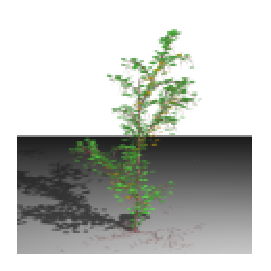
\includegraphics[height=4cm,width=3.5cm, angle=0]{images/clone0}
        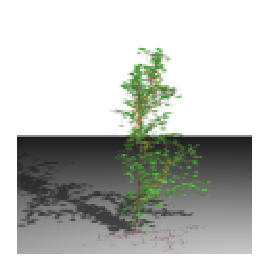
\includegraphics[height=4cm,width=3.5cm, angle=0]{images/clone1}
        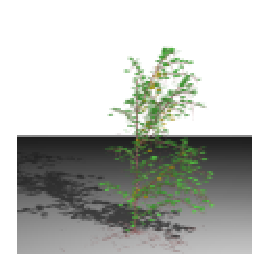
\includegraphics[height=4cm,width=3.5cm, angle=0]{images/clone2}
        \caption{Different clones originating from the same mother}
        \label{fig:clones}
\end{figure}
Assuming that a region have similar properties, it is sufficient to simulate
only one tree, making state snapshots of it at different stages of
development. Consider these trees as a mother set which is used to spawn
clones, by simply changing the random seeds of the branches. To make further
adjustments, parameters as position can be tilted to make the trees
personalized.


\subsubsection{Underlying language specific conceptual issues}
To optimize performance it is needful to utilize destructively mutable arrays
in which to store the branch states. There are several approaches to make this
happen.
\paragraph{ST Monad}
Working in the State-Transformer monad allows for use of the STArray. The STArray 
may however not be exported from the ST monad (to an unstrict environment).
Thus, all array-action must take place within the ST monad, exporting only the
result in a safe form. If the simulation takes place within the ST Monad, no
communication can be done from the outside to the simulation engine. The
resulting simulation is trapped inside ST and exports geometric data in an
infinite list. From the outside the list is pulled and desired models are sent
down the graphics step. Since ST is strict, all geometric data is computed,
not only the one that is used. This is highly undesirable.
\\\\
It is possible to freeze an STArray and thereby converting it to an ordinary
non-strict immutable haskell array. That may in its turn be thawed to an
STArray again within the ST monad, allowing for further use. This can be done
without making copies, using the 'unsafe' operations. It was therefore decided
to remain outside ST everywhere except where it is absolutely necessary, that
is in the inner simulation loop.

\subsection{Visualization}
\subsubsection{Intermediate representation}
In order to visualize a simulation, the simulation representation is first
converted into an intermediate construction, that holds the key properties of
the geometric representation. The intermediate representation may then be
exported to specific standards, such as an OpenGL render section or a collection
of raytracable objects for use with povray or such.

\subsubsection{Processing the Simulated representation}
The simulation representation is constituted of a tree-structure, corresponding
to the actual tree. Therefor, conversion starts at the root, recursively
climbing the branches while updating position and direction of the current
branch. Each branch is represented with a set of cones, whose element count
determines the geometric resolution of the branch. 

\subsubsection{Branch properties}
The thickness of a branch has been decided by the simulation stage, but the
geometry builder makes decisions about how the branch will thin out towards its
end.

\subsubsection{Geometrical resolution}
Obviously, the desired
resolution will vary greatly, depending on closest distance to camera, occluding
geometry and most important - the gradient, or the changing of direction along 
the branch. The constructor will thus increase geometrical resolution when the 
shape is irregular and decrease when the shape tends to be uniform. Leaves are
represented with a simple polygonal surface, with a texture reflecting the
prosperity of the leaf (dying leave are typically low on chlorophyll and thus
yellow or brown in contrast to healthy green).




% Analysis, results, usefulness, ...

\section{Comparison of methodologies}


\subsection{Global analysis}


    The  parameterized approach makes use of its global view of the
    tree for a number of reasons. The ability to maintain a strict
    shape and to apply restriction of growth relies on such
    information. Further more, it is necessary to access such
    information when emulating forces of nature. For instance the sun
    emulation is dependent on information of the neighbouring
    branch-environment.

    While possible to some extent, global analysis is generally
    avoided and discouraged with the monadic approach due to the
    complexity and dependencies it causes. Thus some designs and
    behaviours are hard to model, such as advanced resource
    distributions or forcing a certain shape on a plant in the
    presence of resource limitations.


\subsection{Extensibility}

    When attempting to model a plant that is out-of-structure with the
    parametrized system there is need to make changes in some of the
    underlying layer. In the most probable cases it will be enough to
    extend the metalanguage, but severe differences need a change in
    the simulation module. The monadic approach uses a much simpler
    and less hardcoded simulationfunction with most of the logic in
    the actual plant descriptions, allowing extensions to be coded
    completely by the user. However, the relatively primitive language
    may limit the complexity of feasible additions, especially if they
    involve global analysis.

\newpage
\section{Results}

    We successfully simulate a large number of trees within reasonable
    time. They can be simulated in real-time, should the structure not
    be complex, or quasi-realtime when necessary. Further more, it is
    possible to export geometrical representations to be used with
    raytracers for high-quality images.
    







\appendix


\section{Monadic Approach - Examples}

\label{monadic_examples}

    This section contains a number of more advanced examples, to give
    a taste of the possibilities of the system. 







      


\section{Database Approach - Examples}

    This section is meant to explain how to model a tree after ones liking,
    using the database-approach. As stated priviously, the seed is determined by
    a stream of (interface, node) tuples which define the branching/leaf-levels
    of the tree.

\subsection{Basemodel}

    To start off, a base-tree is considered from which specialized instances
    will be derived. \\
                                             
\begin{tabular}{ll}
  &StdEarth\\
  <<.&(strif, strbranch)\\
  .<<&(leafif 0.1, stdleaf 1.0 1.1)\\
\end{tabular}
 
\begin{figure}[htb]
        \centering
        \includegraphics[height=4cm,width=4cm, angle=0]{images/dbex0}
        \caption{The basic building-blocks}
        \label{fig:graph2}
\end{figure}

    Only two levels, one trunk and one leafnode results in the above image,
    using simple standard components, \emph{strif, strbranch} and the
    leaf-components \emph{leafif} (leaf interface) and \emph{stdleaf} which
    simply takes the size and a development parameter.

\subsubsection{Adding branches}

    Adding branches by placing a branch-level between the existing ones.

\begin{tabular}{ll}
  &StdEarth\\
  .<<&(if\_setdist (dist\_root 10.0 29.1) \$ strif,\\
  &br\_setthick 0.2 \$ strbranch)\\
  <<&(angif 90 0,\\
  &br\_setthick 0.2 \$ strbranch)\\
  <<.&(if\_setevol (efnc\_param 0.05 0.0) \$ leafif 0.5,\\
  &stdleaf 4.0 0.10)\\
\end{tabular}

\begin{figure}[htb]
        \centering
        \includegraphics[height=4cm,width=4cm, angle=0]{images/dbex1}
        \caption{Another branch-level added}
        \label{fig:graph3}
\end{figure}

    Branches appear from the trunk and carries the leaf into the surrounding.
    Also note that the \emph{if\_setdist} sets the distribution function, that
    is the function that says how power will be distributed on a certain level.
    the \emph{br\_setthick} sets the thickness of certain branch-level.

\subsubsection{Randomize}

    The branch interfaces have this far been static and will now be randomized.
    More branch-levels are added.

\begin{tabular}{ll}
    &StdEarth\\
    .<<&(if\_setdist (dist\_root 10.0 29.1) \$ strif,\\ 
    &br\_setthick 0.2 \$ ranagebranch 0.3 0.0)\\
    <<&(if\_setmod (mdfnc\_rlen 0.7)  \$ \\
    &if\_setevol (efnc\_param 0.5 0.2) \$ \\
    &if\_setdist (dist\_shaped 1.4 (\_->1.0) (16.0, 0.1) ) \$ \\
    &angifi 20 45 , \\
    &br\_setthick 0.1 \$ ranwigbranch 0.5 0.2)\\
    <<&(if\_setmod (mdfnc\_mplen 0.7)  \$ \\
    &if\_setevol (efnc\_param 0.14 0.01) \$ \\
    &if\_setdist (dist\_shaped 0.3 (\_->1.0) (7.0,1.0)) \$ \\
    &angifi 35 55 , \\
    &br\_setthick 0.1 \$ ranwigbranch 0.5 0.4) \\
    <<.&(if\_setevol (efnc\_param 0.05 0.0) \$ leafif 0.5, \\
    &stdleaf 4.0 0.10) \\
 
\end{tabular}

\begin{figure}[htb]
        \centering
        \includegraphics[height=4cm,width=4cm, angle=0]{images/dbex2}
        \caption{Randomization and some modifications added}
        \label{fig:graph4}
\end{figure}

    The \emph{if\_setmod} sets a restriction on the power distributed from a
    certain level. \emph{mdfnc\_rlen 0.7} says that a child cannot grow beyond
    0.7 times the relative growth of its mother. The \emph{if\_setevol} sets the
    evolution paramaters for a level, that is when it is going to spawn. Using
    ranwigbranch a complex multi-period sine-shape is applied to the branches.
    The \emph{if\_setshaped} is used to set the shape of a level. Typically on
    the trunk-level a certain shape is defined. For columnar trees such as this
    example, it may simply by a \emph{lambda}->1.0 to say that it branches should be
    equally intensified over the trunk, while some trees might have more of a
    pyramid or even wavy shape. The \emph{angifi x y} says that a branch will
    spawn with an angle of x +/- y in relation to its mother. 

\subsubsection{Further improvements}

    Adding more levels and fine-tuning the parameters gives further improvements
    to the scene.\\

\begin{tabular}{ll}
  &StdEarth\\
  .<<&(if\_setdist (dist\_root 10.0 29.1) \$ strif,\\
  &br\_setthick 0.1 \$ ranagebranch 0.3 0.0)\\
             
         <<&(if\_setmod (mdfnc\_rlen 0.7)  \$\\ 
           &if\_setevol (efnc\_param 0.5 0.2) \$\\ 
           &if\_setdist (dist\_shaped 1.4 f0 (16.0, 0.1) ) \$\\ 
           &angifi 20 45 ,\\ 
           &br\_setthick 0.1 \$ ranwigbranch 0.5 0.2)\\

         <<&(if\_setmod (mdfnc\_mplen 0.7)  \$ \\
           &if\_setevol (efnc\_param 0.14 0.01) \$ \\
           &if\_setdist (dist\_shaped 0.3 f0 (7.0,1.0)) \$ \\
           &angifi 35 55 , \\
           &br\_setthick 0.1 \$ ranwigbranch 0.5 0.4) \\
             
         <<&(if\_setmod (mdfnc\_mplen 0.1 ) \$ \\
           &if\_setevol (efnc\_param 0.05 0.005) \$ \\
           &if\_setdist (dist\_shaped 0.3 f0 (3.0,1.0)) \$ \\
           &angifi 45 65, \\
           &br\_setthick 0.1 \$ ranwigbranch 0.5 0.9) \\
         <<.&(if\_setevol (efnc\_param 0.05 0.0) \$ leafif 0.05, \\
            &stdleaf 4.0 0.10) \\
	
\end{tabular}


\begin{figure}[htb]
        \centering
        \includegraphics[height=4cm,width=4cm, angle=0]{images/dbex3}
        \caption{Randomization and some modifications added}
        \label{fig:graph5}
\end{figure}



      




% \newpage
\begin{thebibliography}{MMM}
% Definiera k�lla med:  \bibitem{key} F�rfattare. \textsl{Titel}. F�rlag, �r etc..
% referera sedan med \cite{key}
% exempel:
\bibitem{prusin_animplant} Przemyslaw Prusinkiewicz, Mark Hammel, Eric Mjolsness. \textsl{Animation of Plant Development.} 1993
\bibitem{povray} Povray, \textsl{Persistence of Vision Ray-Tracer}, \texttt{http://www.povray.org}
\bibitem{alexis} Alexis Brandeker \textsl{The Fractal Structure of Interstellar Clouds} 1998
\bibitem{lsys_theory_vis} Przemyslaw Prusinkiewicz, \textsl{L-Systems: From the theory to visual models of plants} 1996
\bibitem{obs_sharing} Koen Claessen, David Sands, \textsl{Observable Sharing for Functional Circuit Description}
\end{thebibliography}


\end{document}




